\documentclass[12pt,a4paper]{report}
\usepackage[utf8]{inputenc}
\usepackage{amsmath}
\usepackage{amsfonts}
\usepackage{amssymb}
\usepackage{graphicx}
\usepackage{listings}
\usepackage{color}

\definecolor{mygreen}{rgb}{0,0.6,0}
\definecolor{mygray}{rgb}{0.5,0.5,0.5}
\definecolor{mymauve}{rgb}{0.58,0,0.82}

\lstset{ %
  backgroundcolor=\color{white},   % choose the background color; you must add \usepackage{color} or \usepackage{xcolor}
  basicstyle=\footnotesize,        % the size of the fonts that are used for the code
  breakatwhitespace=false,         % sets if automatic breaks should only happen at whitespace
  breaklines=true,                 % sets automatic line breaking
  captionpos=b,                    % sets the caption-position to bottom
  commentstyle=\color{mygreen},    % comment style
  deletekeywords={...},            % if you want to delete keywords from the given language
  escapeinside={\%*}{*)},          % if you want to add LaTeX within your code
  extendedchars=true,              % lets you use non-ASCII characters; for 8-bits encodings only, does not work with UTF-8
  frame=single,                    % adds a frame around the code
  keepspaces=true,                 % keeps spaces in text, useful for keeping indentation of code (possibly needs columns=flexible)
  keywordstyle=\color{blue},       % keyword style
  language=Java,                 % the language of the code
  otherkeywords={*,...},            % if you want to add more keywords to the set
  numbers=left,                    % where to put the line-numbers; possible values are (none, left, right)
  numbersep=5pt,                   % how far the line-numbers are from the code
  numberstyle=\tiny\color{mygray}, % the style that is used for the line-numbers
  rulecolor=\color{black},         % if not set, the frame-color may be changed on line-breaks within not-black text (e.g. comments (green here))
  showspaces=false,                % show spaces everywhere adding particular underscores; it overrides 'showstringspaces'
  showstringspaces=false,          % underline spaces within strings only
  showtabs=false,                  % show tabs within strings adding particular underscores
  stepnumber=2,                    % the step between two line-numbers. If it's 1, each line will be numbered
  stringstyle=\color{mymauve},     % string literal style
  tabsize=2,                       % sets default tabsize to 2 spaces
  title=\lstname                   % show the filename of files included with \lstinputlisting; also try caption instead of title
}
\begin{document}
\begin{lstlisting}
package validation

import Configurator.BinaryConstraint
import Configurator.BinaryOperator
import Configurator.BooleanLiteral
import Configurator.DoubleLiteral
import Configurator.IntLiteral
import Configurator.Literal
import Configurator.Parameter
import Configurator.ParameterIdentifier
import Configurator.StringLiteral
import Configurator.UnaryConstraint
import org.eclipse.emf.ecore.EObject

class Constraints {
	
	// Constraint operator contraint
	def static dispatch boolean constraint(BinaryConstraint it) {
		(andOrOperatorConstraint(it)) || (mathOperatorConstraint(it))
	}
	
	def static boolean mathOperatorConstraint(BinaryConstraint it) {
		(operator.equals(BinaryOperator.NOTEQUALS) || operator.equals(BinaryOperator.EQUALS) || operator.equals(BinaryOperator.GT) || operator.equals(BinaryOperator.GTEQ) || operator.equals(BinaryOperator.LT) || operator.equals(BinaryOperator.LTEQ)) 
		&& 
		(leftOperand instanceof ParameterIdentifier || leftOperand instanceof Literal)
		&&
		(it.rightOperand instanceof ParameterIdentifier || it.rightOperand instanceof Literal)
	}
	
	def static boolean andOrOperatorConstraint(BinaryConstraint it) {
		(operator.equals(BinaryOperator.AND) || operator.equals(BinaryOperator.OR) || operator.equals(BinaryOperator.XOR))
		&&
		(leftOperand instanceof BinaryConstraint || leftOperand instanceof UnaryConstraint)
		&&
		(rightOperand instanceof BinaryConstraint || rightOperand instanceof UnaryConstraint)
	}
	
	// Parameter can only have either literal or enum value
	def static dispatch boolean constraint(Parameter it) {
		(literalValues == null && enumValue != null && enumCountConstraint) 
		||
		(literalValues != null && enumValue == null && literalTypesConstraint && literalCountConstraint) 
	}
	
	def static boolean literalCountConstraint(Parameter it) {
		(literalValues.size <= maxChosenValues) && (literalValues.size >= minChosenValues)
	}
	
	def static boolean enumCountConstraint(Parameter it) {
		(enumValue.size <= maxChosenValues) && (enumValue.size >= minChosenValues)
	}
	
	// Literal values need to be of the same type.
	def static boolean literalTypesConstraint(Parameter it) {
		literalValues.forall[x | x instanceof IntLiteral]
		||
		literalValues.forall[x | x instanceof StringLiteral]
		|| 
		literalValues.forall[x | x instanceof DoubleLiteral]
		||
		literalValues.forall[x | x instanceof BooleanLiteral]
	}	
	
	// Unary constraint can only contains binary constraint	
	def static dispatch boolean constraint(UnaryConstraint it) {
		operand instanceof BinaryConstraint
	}
	
	// Catch all case for dynamic dispatch resolution
	def static dispatch boolean constraint(EObject it) {
		true
	}
}
\end{lstlisting}
\newpage
\begin{figure}[h!]
%  \caption{A picture of a gull.}
\centering
    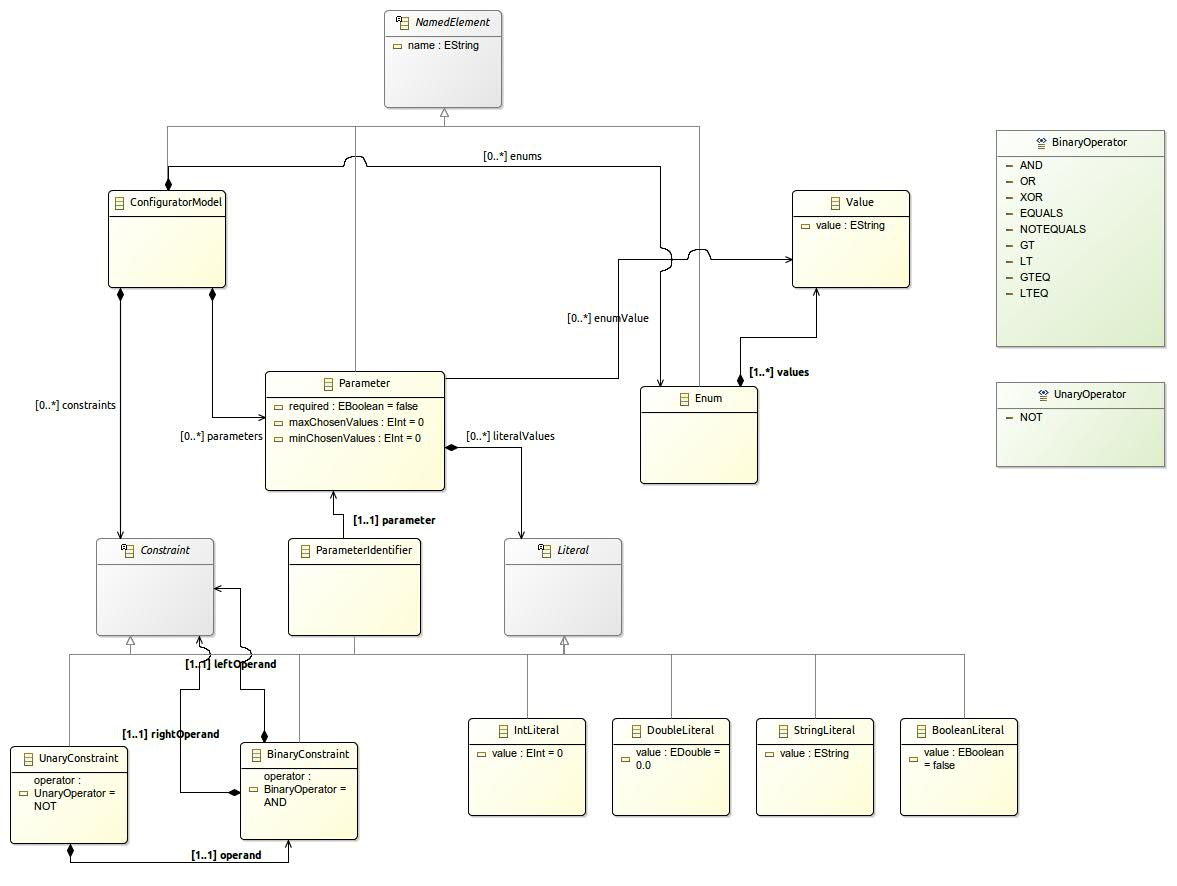
\includegraphics[width=1.2\textwidth]{class_diagram.jpg}
\end{figure}
\end{document}